\section{Opis i treść kodu PythonPIC}\label{sec:code}
Cały kod programu w celu ułatwienia jego użycia i reprodukowalności wyników tworzony był i jest
dostępny\footnote{\url{https://github.com/StanczakDominik/PythonPIC}} na platformie GitHub.

Program ma obiektową strukturę zewnętrzną, którą w celu łatwości
zrozumienia jego działania nakrywa wewnętrzną warstwę składającą się
głównie z n-wymiarowych tablic \code{numpy.ndarray} oraz zwektoryzowanych
operacji na nich.

Część symulacyjna kodu składa się z kilku prostych koncepcyjnie elementów:

\subsection{Grid --- siatka Eulera}
Klasa reprezentująca dyskretną siatkę Eulera, na której dokonywane są
obliczenia dotyczące pól elektromagnetycznych oraz gęstości ładunku i
prądu. Zawiera dane historyczne dotyczące wielkości na siatce
i linki do plików \code{.hdf5} przechowujących te wielkości.
Posiada dwie subklasy do praktycznych zastosowań w różnego rodzaju
symulacjach: \code{PeriodicGrid} oraz \code{NonperiodicGrid}.

Zawiera następujące parametry:
\begin{itemize}
    \itemi{} $x_i$ --- tablicę położeń lewych krawędzi komórek siatki
    \itemi{} $N_G$ --- liczbę komórek siatki
    \itemi{} $T$ --- sumaryczny czas trwania symulacji
    \itemi{} $\Delta x$ --- krok przestrzenny siatki --- $N_G \Delta x$ daje
        długość obszaru symulacji
    \itemi{} $\rho_i$ --- tablicę gęstości ładunku na siatce.
    \itemi{} $\vec{j}_{i,j}$ --- tablicę gęstości prądu na siatce.
    \itemi{} $E_{i,j}, B_{i,j}$ --- tablice pól elektrycznego i magnetycznego na siatce.
    \itemi{} $c$, $\varepsilon_0$ --- stałe fizyczne --- prędkość światła oraz
        przenikalność elektryczną próżni.
    \itemi{} $\Delta t$ --- krok czasowy symulacji, obliczony jako $\Delta t =
        \Delta x / c$.
    \itemi{} $N_T$ --- liczbę iteracji czasowych symulacji.
    \itemi{} \code{BC} --- \english{Boundary Condition}, obiekt zawierający informacje dotyczące
        warunku brzegowego zadanego na pole elektryczne i magnetyczne. W przypadku symulacji
        laserowej jest to instancja klasy \code{Laser} zawierająca informacje o
        długości fali, kształcie obwiedni
        i polaryzacji impulsu. W każdej iteracji \code{BC} poprzez metodę
        \code{apply} aktualizuje wartości na lewym brzegu siatki obliczeniowej.
\end{itemize}

Istotne metody klasy \code{Grid}, o których należy wspomnieć, to:
\begin{itemize}
     \itemi{} \code{apply\_bc} --- aktualizuje krańcowe wartości tablic $E$, $B$
         w oparciu o podany warunek brzegowy (\code{BC}).
     \itemi{} \code{gather\_current} --- zbiera ładunek z cząstek na siatkę
     \itemi{} \code{gather\_charge} --- zbiera prąd z cząstek na siatkę
     \itemi{} \code{init\_solve} --- uruchamia początkową, spektralną iterację obliczającą równowagowe
           pole elektrostatyczne na podstawie gęstości ładunku z cząstek
     \itemi{} \code{solve} --- uruchamia iterację ewolucji czasowej pola elektromagnetycznego na podstawie
           prądów w symulacji
     \itemi{} \code{field\_function} --- interpoluje pola elektryczne i magnetyczne do danych położeń, używane
           do obliczenia pól w cząstkach
     \itemi{} \code{save\_field\_values} --- zapisuje dane dotyczące wartości historycznych na siatce w danej iteracji.
           Należy zaznaczyć, że wielkości na komórkach granicznych nie są zapisywane.
     \itemi{} \code{postprocess} --- przetwarza zebrane w czasie symulacji minimalne informacje dotyczące pól, prądów i ładunków
           na informacje dotyczące energii
\end{itemize}

\subsection{Species --- cząstki}
Klasa reprezentująca pewną grupę makrocząstek o wspólnych cechach, takich
jak ładunek bądź masa.  Przykładowo, w symulacji oddziaływania lasera z
tarczą wodorową jedną grupą są protony, zaś drugą --- elektrony.  Do
zainicjalizowania wymaga instancji \code{Grid}, z której pobiera informacje
takie jak stałe fizyczne $c$, $\varepsilon_0$, liczbę iteracji czasowych
$N_T$ i czas trwania iteracji $\Delta t$.

Zawiera skalary:
\begin{itemize}
    \itemi{} $N$ --- liczba makrocząstek
    \itemi{} $q$ --- ładunek cząstki
    \itemi{} $m$ --- masa cząstki
    \itemi{} \code{scaling} --- liczba rzeczywistych cząstek, jakie reprezentuje
        sobą makrocząstka. Jej sumaryczny ładunek wynosi $q *
        $\code{scaling}, masa $m * $\code{scaling}.
    \itemi{} \code{N\_alive} --- liczba cząstek obecnie aktywnych w symulacji.
        Zmniejsza się w miarę usuwania cząstek przez warunki brzegowe.
\end{itemize}

Poza skalarami zawiera tablice rozmiaru $N$:
\begin{itemize}
    \itemi{} jednowymiarowych położeń makrocząstek $x^n$, zapisywanych w
        iteracjach $n, n+1, n+2$\ldots
    \itemi{} trójwymiarowych prędkości makrocząstek $\vec{v}^{n+\frac{1}{2}}$,
        zapisywanych w iteracjach $n+\frac{1}{2}, n+\frac{3}{2}, n+\frac{5}{2}$\ldots
    \itemi{} stanu makrocząstek (flagi oznaczające cząstki aktywne
        bądź usunięte z obszaru symulacji)
\end{itemize}

Poza tym, zawiera też informacje dotyczące zbierania danych diagnostycznych
dla cząstek, niepotrzebnych bezpośrednio w czasie symulacji:
\begin{itemize}
    \itemi{} \code{name} --- słowny identyfikator grupy cząstek, dla potrzeb legend wykresów
    \itemi{} $N_T$ --- liczbę iteracji czasowych w symulacji
    \itemi{} $N_T^s$ --- zmniejszoną liczbę iteracji, w których następuje pełne
        zapisanie położeń i prędkości cząstek.  Dane te są wykorzystywane
        do tworzenia diagramów fazowych cząstek.
    \itemi{} odpowiadające poprzednio wymienionym tablice rozmiaru $(N_T^s,
        N)$, $(N_T^s, N, 3)$. 
    \itemi{} jedną tablicę rozmiaru $(N_T, N_G)$ dotyczącą zebranych podczas
        depozycji ładunku informacji diagnostycznych o przestrzennej gęstości cząstek.
    \itemi{} trzy tablice rozmiaru $(N_T)$ dotyczącą średnich prędkości,
        średnich kwadratów prędkości i odchyleń standardowych prędkości.
\end{itemize}

Jeżeli liczba makrocząstek lub iteracji przekracza pewną stałą (rzędu $10^4$), dane zapisywane są jedynie dla co $n$-tej cząstki,
gdzie $n$ jest najniższą liczbą całkowitą która pozwala na zmniejszenie tablic poniżej tej stałej.

Warto wspomnieć o następujących metodach klasy \code{Species}:
\begin{itemize}
    \itemi{} \code{apply\_bc} --- aplikuje warunki brzegowe. W symulacjach okresowych jest to przywrócenie cząstek do rejonu symulacji ($x := x \% L$), w symulacjach nieokresowych usunięcie ich.
    \itemi{} \code{position\_push}  --- przemieszcza cząstki w przestrzeni.
    \itemi{} \code{velocity\_push} --- interpoluje pola do pozycji cząstek i aktualizuje ich prędkości na podstawie integratora Borysa.
    \itemi{} \code{save\_particle\_values} --- zapisuje wartości danych historycznych cząstek.
    \itemi{} \code{distribute\_uniformly} --- rozmieszcza cząstki równomiernie na zadanym przedziale
    \itemi{} \code{distribute\_nonuniformly} --- rozmieszcza cząstki według zadanej funkcji rozkładu gęstości
\end{itemize}

Poza tym \code{Species} zawiera również rozmaite metody służące inicjalizacji
prędkości i położeń przy pomocy zaburzeń sinusoidalnych bądź losowych.

\subsection{Simulation}
Klasa zbierająca w całość \code{Grid} oraz dowolną liczbę \code{Species} zawartych w
symulacji, jak również pozwalająca w prosty sposób na wykonywanie iteracji
algorytmu i analizy danych. Jest tworzona tak przy uruchamianiu symulacji,
jak i przy wczytywaniu danych z plików \code{.hdf5}.

\begin{itemize}
    \itemi{} $\Delta t$ --- krok czasowy
    \itemi{} $N_T$ --- liczba iteracji w symulacji
    \itemi{} \code{Grid} --- obiekt siatki
    \itemi{} \code{list\_species} --- lista grup makrocząstek w symulacji
\end{itemize}

Przygotowanie warunków początkowych do danej symulacji polega na utworzeniu
nowej klasy dziedziczącej po \code{Simulation}, która przygotowuje siatkę,
cząstki i warunki brzegowe zgodnie z założeniami eksperymentu i wywołuje
konstruktor \code{Simulation}.  Należy również przeciążyć metodę
\code{grid\_species\_initialization}, która przygotowuje warunki początkowe.
Domyślna wersja tej metody wykonuje pierwszą, początkową iterację równań ruchu
przesuwającą prędkość o $-\Delta t / 2$ w tył. To zaś pozwala na zachowanie
symplektyczności integratora, co pomaga zachować energię w symulacji.  W tym
momencie jest też tworzony plik \code{.hdf5}, do którego zapisywane są dane
gromadzone w czasie symulacji.

Aby uruchomić symulację, należy wywołać jedną z metod:
\begin{itemize}
     \itemi{} \code{run} --- podstawowy cykl obliczeń, używany do pomiarów
         wydajności programu
     \itemi{} \code{test\_run} --- obliczenia oraz obróbka danych na potrzeby
         analizy, głównie stosowana w testach
     \itemi{} \code{lazy\_run} --- \code{test\_run} z zapisem do pliku oraz
         wczytaniem z pliku \emph{.hdf5}, jeżeli początkowe warunki oraz
         wersja kodu zgadzają się. W przeciwnym razie symulacja zostaje
         uruchomiona na nowo.
\end{itemize}

\subsection{Pliki pomocnicze}
Poza powyższymi program jest podzielony na pliki z implementacjami algorytmów numerycznych,
co ułatwia kompilację JIT, pozwala na zwiększenie niezależności testów oraz
zwiększa modularność kodu.
\begin{itemize}
    \itemi{} \code{BoundaryCondition} --- implementacja warunków brzegowych
    \itemi{} \code{charge\_deposition} --- depozycja ładunku na siatkę
    \itemi{} \code{current\_deposition} --- depozycja prądu podłużnego i poprzecznego na siatkę
    \itemi{} \code{density\_profiles} --- profile przestrzenne kształtów preplazmy
        oraz algorytmy rozkładające cząstki według tych rozkładów.
    \itemi{} \code{FieldSolver} --- spektralne i rotacyjne algorytmy rozwiązywania równań Maxwella na siatce Eulera.
    \itemi{} \code{particle\_push} --- implementacja integratorów równań ruchu typu \english{leapfrog} oraz Borysa.
    \itemi{} \code{field\_interpolation} --- interpolacja pól elektromagnetycznych z położeń na siatce do cząstek.
\end{itemize}

Katalog \code{visualization} zawiera wizualizacje danych.
\begin{itemize}
    \itemi{} \code{animation} --- tworzy animacje dla celów analizy danych
    \itemi{} \code{time\_snapshots} --- implementacje wykresów zależnych od czasu, ilustrujących stan symulacji w danej iteracji.
    \itemi{} \code{static\_plots} --- tworzy statyczne wykresy dla celów analizy danych
    \itemi{} \code{plotting} --- zawiera ustawienia dotyczące analizy danych
\end{itemize}

Przygotowane konfiguracje istniejących symulacji są zawarte w katalogu 
\code{configs}, zaś algorytmiczne testy jednostkowe są zawarte w katalogu \code{tests}.

\subsection{Wykorzystane biblioteki Pythona}

Pomijamy tutaj bibliotekę standardową jako wbudowaną w sam język, skupiając się na przydatnych bibliotekach zewnętrznych.

\subsubsection{Numpy}
\code{numpy}\cite{numpy} to biblioteka umożliwiająca wykonywanie złożonych obliczeń na
n-wymiarowych macierzach bądź tablicach, utworzona w celu umożliwienia
zastąpienia operacjami wektorowymi iteracji po tablicach, powszechnie
stosowanych w metodach numerycznych i będących znanym słabym punktem
Pythona.

Pod zewnętrzną powłoką zawiera odwołania do znanych, wypróbowanych i
sprawdzonych w nauce modułów \code{LAPACK}, \code{BLAS} napisanych w
szybkich, niskopoziomowych językach C oraz \code{FORTRAN}.  Jest to
\emph{de facto} standard większości obliczeń numerycznych w Pythonie.

Należy zauważyć, że operacje matematyczne w wersji \code{numpy} zawartej
w popularnej dystrybucji Anaconda są automatycznie zrównoleglane tam, gdzie
pozwala na to niezależność obliczeń dzięki dołączonym bibliotekom Intel Math
Kernel Library.\cite{intel-mkl} 

Numpy jest oprogramowaniem otwartym, udostępnianym na licencji BSD\@.


\subsubsection{scipy}
Kolejną podstawową biblioteką w numerycznym Pythonie jest \code{scipy}\cite{scipy},
biblioteka zawierająca wydajne gotowe implementacje wielu powszechnych algorytmów
numerycznych służących między innymi całkowaniu, optymalizacji funkcji rzeczywistych,
uczeniu maszynowemu, algebrze liniowej czy transformatom Fouriera.

\subsubsection{Numba}
\code{numba} to biblioteka służąca do kompilacji just-in-time wysokopoziomowego
kodu Pythona do kodu niskopoziomowego przy pierwszym uruchomieniu programu. W
wielu przypadkach pozwala na osiągnięcie kodem napisanym w czystym Pythonie
wydajności marginalnie niższej bądź nawet równej do analogicznego programu w C
bądź Fortranie.~\cite{numba}

Jednocześnie należy zaznaczyć prostotę jej użycia. W wielu przypadkach wystarczy
dodać do funkcji dekorator \code{@numba.jit}:

\lstinputlisting[language=Python, numbers=left, caption=Przykład zastosowania kompilacji just-in-time z biblioteki Numba wykorzystujący metody pomiaru czasu środowiska Jupyter.]{listings/numba_example.py}

Istniejącym od niedawna kodem symulacyjnym implementującym tą metodę jest FBPIC\cite{fbpic}.


\subsubsection{HDF5}
HDF5 jest wysokowydajnym formatem plikow służącym przechowywaniu danych
liczbowych w drzewiastej, skompresowanej strukturze danych, razem z
równoległym, wielowątkowym zapisem tych danych.  W Pythonie implementuje go
biblioteka h5py\cite{h5py}.

W bieżącej pracy wykorzystuje się go do przechowywania danych liczbowych
dotyczących przebiegu symulacji, pozwalających na ich dalsze przetwarzanie
i analizę poprzez wizualizację.

\subsubsection{matplotlib}
Do wizualizacji danych z symulacji (oraz tworzenia schematów w sekcji
teoretycznej niniejszej pracy) użyto własnoręcznie napisanych skryptów w
uniwersalnej bibliotece graficznej \code{matplotlib}\cite{matplotlib}.
\code{matplotlib} zapewnia wsparcie zarówno dla grafik statycznych w różnych układach
współrzędnych (w tym 3D), jak również dla dynamicznie generowanych animacji
przedstawiających przebiegi czasowe symulacji.

\subsubsection{py.test}
Przy pracy nad kodem użyto frameworku testowego \code{py.test}~\cite{pytest}.
Tworzenie testów jest trywialne:

\lstinputlisting[language=Python, numbers=left, caption=Podstawowy przykład testu w pliku \code{func.py}]{listings/func.py}

Uruchamianie zaś:

\begin{lstlisting}[language=Bash]
    >>> pytest func.py
    === FAILURES ===
    ___failing ___

        def test_failing():
    >       assert f(4) == 13
    E       assert 12 == 13
    E        +  where 12 = f(4)

    func.py:10: AssertionError
    === 1 failed, 1 passed in 0.10 seconds ===
\end{lstlisting}

Należy zaznaczyć, że w symulacjach numerycznych, gdzie błędne działanie programu nie
objawia się zazwyczaj formalnym błędem, a jedynie błędnymi
wynikami, dobrze zautomatyzowane testy jednostkowe potrafią zaoszczędzić
bardzo dużo czasu na debugowaniu poprzez automatyzację uruchamiania
kolejnych partii kodu i lokalizację błędnie działających części algorytmu.
Dobrze napisane testy są praktycznie koniecznością w dzisiejszych czasach,
zaś każdy nowo powstały projekt symulacyjny powinien je
wykorzystywać, najlepiej do weryfikacji każdej części algorytmu z osobna.

Dobrym przykładem skutecznego testu jednostkowego jest porównanie energii kinetycznej
elektronu o znanej prędkości z wartością tablicową, zawarte jako test w pliku
\code{pythonpic/tests/test\_species.py}.

\code{py.test} jest oprogramowaniem otwartym, dostępnym na licencji MIT\@.

\subsubsection{Travis CI}
Nieocenionym narzędziem w pracy nad kodem był system ciągłej integracji
(\emph{continuous integration}) Travis CI~\cite{travisci}
dostępny za
darmo dla projektów open-source. Travis pobiera aktualne wersje kodu przy
każdej aktualizacji wersji dostępnej na serwerze GitHub i uruchamia testy,
zwracając komunikat o ewentualnym niepowodzeniu i pozwalając na jednoczesne
uruchamianie bieżących, intensywnych symulacji przy jednoczesnym
weryfikowaniu w chmurze poprawności działania lżejszych, acz wciąż intensywnych
symulacji testowych i testów algorytmicznych.

\subsubsection{snakeviz}

W optymalizacji przydatny okazał się program \code{snakeviz}\cite{snakeviz} dostępny na
GitHubie i pozwalający na wizualizację wyników z profilowania
symulacji. Pozwala w wygodny sposób zbadać, które fragmenty kodu najbardziej
spowalniają symulację, które są najlepszymi kandydatami do optymalizacji, oraz
jak skuteczne (bądź nieskuteczne) okazują się próby polepszenia ich wydajności.
Działanie programu ilustruje rysunek~\ref{fig:snakeviz}.
\begin{figure}[h!]
  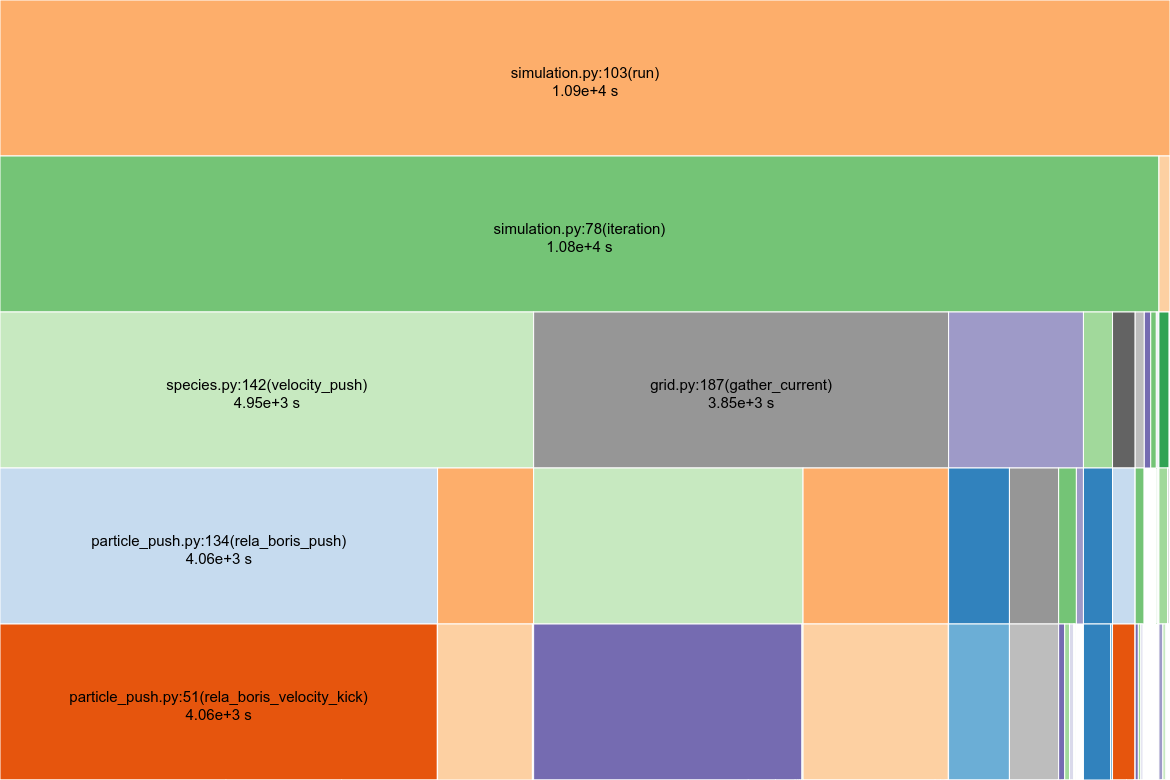
\includegraphics[width=\textwidth]{Images/snakeviz}
  \caption{Wizualizacja szybkości działania poszczególnych fragmentów kodu
    wygenerowana programem \code{snakeviz}.\label{fig:snakeviz}}
\end{figure}
